\documentclass[conference]{IEEEtran}
\usepackage{iftex}
\ifXeTeX
  \usepackage{fontspec}\setmainfont{texgyretermes}[Extension=.otf, UprightFont=*-regular, BoldFont=*-bold, ItalicFont=*-italic, BoldItalicFont=*-bolditalic]
\else
  \usepackage[T1]{fontenc}\usepackage{newtxtext,newtxmath}
\fi
\usepackage{graphicx,booktabs,amsmath,amssymb,cite,url,xcolor,multirow}
\usepackage{tikz}
\usetikzlibrary{positioning,arrows.meta,shapes.geometric,fit,backgrounds}
\input{gen/numbers.tex}
\input{gen/numbers_deep.tex}
\makeatletter\newcommand{\tabinput}[1]{\@@input #1 }\makeatother
\newcommand{\Tone}{T1}\newcommand{\Ttwo}{T2}\newcommand{\Tthree}{T3}\newcommand{\Tfour}{T4}

\begin{document}

\title{Two Shortcuts in the ROAD Masquerade Benchmark\\and How Context Consistency Avoids Them}

\author{\IEEEauthorblockN{Author Name(s) (placeholder)}
\IEEEauthorblockA{Department, Institution (placeholder)\\
City, Country (placeholder)\\
email (placeholder)}}

\maketitle

\begin{abstract}
Masquerade attacks, in which a compromised node silences an electronic control unit and transmits in its place at the correct rate, are the hardest attack class for in-vehicle CAN intrusion detection, and the ROAD dataset is their reference benchmark. ROAD's masquerade captures are simulated by deleting the victim's frames from fabrication captures. We show that this construction leaves two shortcuts. First, a payload shortcut: a per-identifier byte-range rule fitted on attack-free traffic reaches AUC-ROC \ExtAUCmin{} on \NExtCaps{} of the 13 captures, at or above every published unsupervised detector on those attack types. Second, a driving-phase shortcut: supervised deep classifiers learn the scripted manoeuvre that coincides with each attack. On \emph{benign twins}, the same drives with every injected frame removed, they still flag the attack interval (AUC up to \SupTwinMax). We release two counterfactual tests that expose these shortcuts: ROAD-IR, which clamps injected values into their normal range, and the benign twins. We then propose a context-consistency Transformer trained only on attack-free traffic that predicts each identifier's payload from the rest of the bus. As a per-identifier detector it reaches AUC \CtxFourMin--1.00 on four of the five attack types, including the reverse-light attacks that defeat every trivial rule, on both ROAD and ROAD-IR (where the range rule falls to chance), and stays near chance on the benign twins; the single 43-frame coolant capture is unstable across seeds. An identical model without cross-identifier context does not. A cross-corpus check on CrySyS confirms that the payload shortcut is specific to ROAD's construction.
\end{abstract}

\begin{IEEEkeywords}
Controller Area Network, intrusion detection, masquerade attack, benchmark evaluation, shortcut learning, automotive cyber security
\end{IEEEkeywords}

\section{Introduction}
The Controller Area Network (CAN) carries safety-relevant traffic in every modern consumer vehicle, yet it has no sender authentication: any node can transmit any identifier. Intrusion detection systems (IDS) for CAN are therefore an active research area, and they are compared on public datasets. Benchmarks such as Car-Hacking were later shown to be solvable from trivial timing features~\cite{blevins2021,heydari2026}, which moved the field toward ROAD~\cite{verma2024}, a dataset of real, physically verified attacks on a single vehicle.

Within ROAD, the \emph{masquerade} captures are the reference hard case. A masquerade attacker suppresses the legitimate sender and injects forged frames at the original rate, so every timing-based detector fails by construction~\cite{blevins2021}. A line of signal-level detectors has been developed and benchmarked specifically on these captures~\cite{moriano2022,moriano2026jisa,marfo2025,liu2026mids,hegde2026}.

The ROAD authors state, however, that the masquerade captures are \emph{simulated}: they were produced from the fabrication captures by deleting the legitimate frames of the target identifier~\cite{verma2024}. The injected frames themselves are unchanged, and the fabrication attacks inject extreme values (maximum speedometer, maximum coolant temperature). A rule as simple as ``this byte never took this value in normal traffic'' might therefore detect several masquerade captures. If so, scores on the benchmark measure less than the field assumes.

This paper measures that floor, finds a second shortcut that fools learned detectors, and proposes a detector that avoids both. Our contributions are:
\begin{itemize}
\item A payload-level trivial floor for all 13 ROAD masquerade captures, traced byte by byte to the frame-deletion construction. On three of the five attack types it matches or beats published unsupervised detectors~\cite{moriano2026jisa}, and it falls to chance on the independently simulated CrySyS corpus (Sections~\ref{sec:construction}--\ref{sec:abl}).
\item Two counterfactual tests, ROAD-IR (in-range payloads) and benign twins (no attack), which expose a second, driving-phase shortcut learned by supervised deep classifiers (Section~\ref{sec:cf}).
\item A context-consistency Transformer, trained on attack-free traffic only, that detects four of the five attack types, including the reverse-light attacks, with AUC $\geq$\CtxFourMin{} and passes both counterfactual tests, together with the ablation showing that cross-identifier context is what makes it work.
\end{itemize}

\section{Background and Related Work}
\textbf{Attacks.} In a \emph{fabrication} attack, injected frames are added beside the legitimate ones, roughly doubling the identifier's rate. In a \emph{masquerade} attack, the legitimate sender is silenced and only forged frames remain, so the rate is preserved~\cite{verma2024}.

\textbf{Trivial baselines and benchmark audits.} Blevins et al.~\cite{blevins2021} benchmarked time-based IDS on ROAD and showed that simple timing statistics detect injection attacks well; masquerade attacks preserve timing and fall outside their scope. Heydari et al.~\cite{heydari2026} showed that frame-level classifiers on Car-Hacking and Survival exploit identifier shortcuts. Koltai et al.~\cite{koltai2026} found that single-dataset results do not predict cross-dataset performance. None of these establishes a payload-level floor for ROAD masquerade or tests detectors with counterfactual data, a standard tool for exposing shortcut learning in deep networks~\cite{geirhos2020}.

\textbf{Masquerade detectors on ROAD.} Moriano et al.~\cite{moriano2026jisa} benchmark four unsupervised online detectors on the ROAD masquerade captures, namely matrix-correlation distribution (MCD) and correlation (MCC), Ganesan17 (G17)~\cite{ganesan2017} and Moriano22 (M22)~\cite{moriano2022}, under a sliding-window AUC-ROC protocol. Later work applies graph machine learning~\cite{marfo2025}, state-space models~\cite{liu2026mids} and per-identifier residualisation~\cite{hegde2026}. Supervised comparisons~\cite{guerra2024} report near-perfect per-attack scores for an LSTM, and payload-based detectors such as CANdito~\cite{longari2022} model decoded signals. All report absolute scores; none states what a trivial rule achieves on the same captures. Table~\ref{tab:related} summarises the gap.

\begin{table}[t]
\centering
\caption{Closest prior work on ROAD and CAN benchmark auditing.}
\label{tab:related}
\footnotesize
\setlength{\tabcolsep}{3pt}
\begin{tabular}{@{}llll@{}}
\toprule
Work & Data & Features & Trivial floor \\
\midrule
Blevins et al.~\cite{blevins2021} & ROAD & timing & timing only \\
Heydari et al.~\cite{heydari2026} & Car-Hacking, Surv. & ID, payload & not ROAD \\
Koltai et al.~\cite{koltai2026} & 7 CAN datasets & learned & no \\
Moriano et al.~\cite{moriano2026jisa} & ROAD masquerade & signals & no \\
Marfo et al.~\cite{marfo2025} & ROAD masquerade & graph & no \\
Guerra et al.~\cite{guerra2024} & ROAD & ID, payload & no \\
\textbf{This work} & ROAD masquerade & payload & \textbf{yes} \\
\bottomrule
\end{tabular}
\end{table}

\section{The ROAD Masquerade Construction}
\label{sec:construction}
ROAD~\cite{verma2024,roadzenodo} contains 12 ambient captures (about 3\,h) and 33 attack captures from one vehicle on a dynamometer. The 13 masquerade captures cover five attack types: max speedometer (3), max coolant temperature (1), correlated signal (3), reverse light off (3) and reverse light on (3). The authors describe their construction directly: ``Using the fabrication captures we produce simulated masquerade attacks by removing the legitimate target ID frames preceding each injected frame''~\cite{verma2024}. They also list this as a drawback, noting that no un-simulated masquerade data is publicly available.

We confirmed the construction in the data. For every masquerade capture, all non-target traffic is byte-identical to its fabrication twin, and the injected frames match in number up to two frames at the interval edges. Per-frame labels reconstructed from the capture metadata agree exactly with ROAD's own signal-file labels on all 13 captures.

Table~\ref{tab:construction} lists what each attack writes. In three types, the injected byte lies outside the range that byte ever takes in ambient traffic, highway driving included. In the correlated-signal attack, three of the four wheel-speed high bytes are out of range, so the signals are \emph{not} individually plausible. In the reverse-light attacks, byte B2 of identifier 0xD0 only ever takes the values 4 and 12, and the attack writes one of them. The attack toggles the light ``irrespective of the actual gear position''~\cite{moriano2026jisa}, which makes it a context anomaly: a legitimate value at the wrong moment.

\begin{table}[t]
\centering
\caption{Bytes written by each attack (from ROAD metadata) and the range of that byte in ambient traffic. $^\ast$\,=\,value never seen in ambient.}
\label{tab:construction}
\footnotesize
\setlength{\tabcolsep}{3pt}
\begin{tabular}{@{}lp{0.9cm}p{4.6cm}@{}}
\toprule
Attack type & AID & Injected value [ambient range] \\
\midrule
\tabinput{gen/paper_table_construction.tex}
\bottomrule
\end{tabular}
\end{table}

\section{Method}
\label{sec:method}
\textbf{Trivial detectors.} All four are fitted per arbitration identifier (AID) on ambient traffic only, and our code raises an error if an attack capture reaches the fitting path.
\Tone{} (value set) flags a frame if any byte takes a value never seen for that (AID, byte).
\Ttwo{} (range) scores the summed distance of each byte outside its ambient [min,\,max].
\Tthree{} (signal envelope) applies the same test to ROAD's decoded signals.
\Tfour{} (payload novelty) flags a payload tuple never seen for that AID.
Unseen AIDs receive the maximum score.

\textbf{Protocol.} We fit on 10 ambient captures and hold out two (\emph{drive\_basic\_short}, \emph{drive\_extended\_short}) to calibrate thresholds. Frame scores are averaged over 1\,s windows with 0.25\,s stride. As in~\cite{moriano2026jisa}, a window is positive if it overlaps the labelled injection interval, and we report window AUC-ROC. We also report the true-positive rate at the threshold that gives 1\% false positives on the held-out ambient windows (TPR@1\%), with 95\% bootstrap confidence intervals over windows (10{,}000 resamples). Figure~\ref{fig:method} summarises the pipeline.

\textbf{Controls and comparators.} As a learned control we fit one isolation forest per AID on the eight payload bytes (200 trees, three seeds). The code of~\cite{moriano2026jisa} depends on a module that is not in its public repository, so we \emph{quote} its Table~2: per attack type, the mean AUC over its window grid and the best grid cell. The best cell is selected on the test captures and is therefore optimistic. We define \emph{delta-over-trivial} as the best published AUC minus the \Ttwo{} AUC, averaged over the captures of each type.

\begin{figure}[t]
\centering
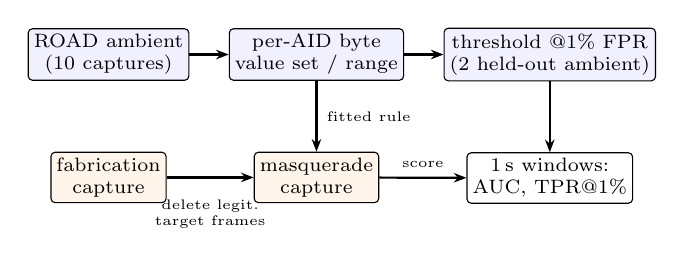
\begin{tikzpicture}[font=\scriptsize, node distance=4mm and 5mm,
  box/.style={draw, rounded corners=1.5pt, align=center, inner sep=2pt, minimum height=6mm, fill=white},
  arr/.style={-{Stealth[length=1.6mm]}, thick}]
\node[box, fill=blue!6] (amb) {ROAD ambient\\(10 captures)};
\node[box, fill=blue!6, right=of amb] (fit) {per-AID byte\\value set / range};
\node[box, fill=blue!6, right=of fit] (thr) {threshold @1\% FPR\\(2 held-out ambient)};
\node[box, fill=orange!8, below=9mm of amb] (fab) {fabrication\\capture};
\node[box, fill=orange!8, below=9mm of fit] (masq) {masquerade\\capture};
\node[box, below=9mm of thr] (win) {1\,s windows:\\AUC, TPR@1\%};
\draw[arr] (amb) -- (fit); \draw[arr] (fit) -- (thr);
\draw[arr] (fab) -- (masq) node[midway, below=1.5mm, font=\tiny, align=center]{delete legit.\\target frames};
\draw[arr] (masq) -- node[midway, above, font=\tiny]{score} (win);
\draw[arr] (fit) -- node[midway, right, font=\tiny]{fitted rule} (masq);
\draw[arr] (thr) -- (win);
\end{tikzpicture}
\caption{Detectors are fitted on attack-free traffic only. ROAD's masquerade captures are fabrication captures with the legitimate target frames deleted, so the injected payloads are unchanged.}
\label{fig:method}
\end{figure}

\section{Results}
\label{sec:results}
\textbf{The floor.} Table~\ref{tab:floor} gives window AUC-ROC per capture. On all \NExtCaps{} speedometer, coolant and correlated-signal captures, the simplest rule (\Ttwo) reaches \ExtAUCmin{}, as do \Tone{} and \Tthree{} with one exception (\Tone{} 0.98 on coolant). At the operating point calibrated on held-out ambient, \Ttwo{} detects \SCTPRmin--\SCTPRmax\% of attack windows on the speedometer and correlated-signal captures. The coolant capture ranks perfectly yet is missed at 1\% FPR: it contains only \CoolantNinj{} injected frames, and its excursion (255 against an ambient maximum of 162) is smaller than benign excursions on other identifiers in the held-out captures. On the extreme-value captures, every fabrication twin scores the same as its masquerade capture (largest difference \FabMasqMaxDiffExt), as the construction predicts. On the \NRlCaps{} reverse-light captures, no trivial rule rises meaningfully above chance (\Ttwo{} \RlAUCmin--\RlAUCmax). Figure~\ref{fig:bytes} shows why: every injected frame of the three extreme types violates the ambient range on exactly the bytes the metadata says were written, and no reverse-light frame does.

\begin{table}[t]
\centering
\caption{Window AUC-ROC of trivial detectors (fitted on ambient only) and the isolation-forest control (IF, mean of 3 seeds) per masquerade capture; TPR@1\%: \% of attack windows detected by \Ttwo{} at 1\% FPR on held-out ambient. Bold: $\geq0.95$.}
\label{tab:floor}
\footnotesize
\setlength{\tabcolsep}{4pt}
\begin{tabular}{@{}lcccccc@{}}
\toprule
Capture & \Tone & \Ttwo & \Tthree & \Tfour & IF & TPR@1\% \\
\midrule
\tabinput{gen/paper_table_floor.tex}
\bottomrule
\end{tabular}
\end{table}

\begin{figure}[t]
\centering
\includegraphics[width=\columnwidth]{gen/fig4_byte_flags.pdf}
\caption{Share of injected frames whose byte lies outside the ambient range of the attacked identifier. The shortcut sits exactly on the bytes written by the attack; reverse-light frames never leave the range.}
\label{fig:bytes}
\end{figure}

\textbf{Against published detectors.} Table~\ref{tab:delta} and Fig.~\ref{fig:floor} compare the floor with~\cite{moriano2026jisa}. On max speedometer, max coolant and correlated signal, the best published detector, even with test-tuned window parameters, ties or trails the range check (delta \DeltaExtMin{} to \DeltaExtMax). On average over its window grid it trails by much more. The published methods earn their keep only on the reverse-light types, where they lead the trivial floor by \DeltaRlMin{} to \DeltaRlMax{}.

\begin{table}[t]
\centering
\caption{Trivial floor (\Ttwo, mean over captures) versus the best of four published unsupervised detectors~\cite{moriano2026jisa} (quoted). Delta = tuned max $-$ \Ttwo.}
\label{tab:delta}
\footnotesize
\setlength{\tabcolsep}{3pt}
\begin{tabular}{@{}lcccc@{}}
\toprule
Attack type & \Ttwo & Published mean & Published max & Delta \\
\midrule
\tabinput{gen/paper_table_delta.tex}
\bottomrule
\end{tabular}
\end{table}

\begin{figure}[t]
\centering
\includegraphics[width=\columnwidth]{gen/fig2_floor_vs_published.pdf}
\caption{Trivial range rule versus the best published detector per attack type~\cite{moriano2026jisa} and the isolation-forest control. Dashes mark the published mean over the window grid.}
\label{fig:floor}
\end{figure}

\textbf{A learned payload model is not a free improvement.} The per-AID isolation forest is weaker than the range rule on the extreme-value types (e.g.\ \IFspeedo{} on speedometer), because one out-of-range byte barely moves a density score over eight bytes. It is the only payload model that separates reverse-light-on (\IFrlOn): the value 12 is rare in ambient traffic and rarely co-occurs with forward-driving bytes. On reverse-light-off it falls below chance (\IFrlOff), because the injected value 4 is the common state.

\section{Ablation and Sensitivity}
\label{sec:abl}
\textbf{Where the signal lives.} Restricting \Ttwo{} to a single byte reproduces the full result on exactly the written bytes (B5 for speedometer and coolant; B0, B2, B6 for correlated signal) and yields chance elsewhere. Ignoring the attacked identifier drops the extreme-value AUCs from 1.00 to \ExclTargetMin--\ExclTargetMax, so physical side-effects in other identifiers carry far less signal than the payload itself. Normalising excursions by range width leaves every AUC unchanged.

\textbf{Robustness.} Figure~\ref{fig:sens} varies the window length (0.25--2\,s) and the share of each ambient capture used for fitting (10--100\%). The extreme-value AUCs never fall below \SensExtMin, so the floor holds with a tenth of the ambient data. Relaxing \Tthree{} to the [p1,\,p99] envelope also leaves them at 0.97 or above. The reverse-light AUCs stay at or below chance throughout.

\textbf{A second corpus.} To test whether the shortcut is specific to ROAD, we apply the identical detectors, without retuning, to the CrySyS dataset~\cite{gazdag2023}. It simulates masquerades on \CryNrec{} benign recordings of another vehicle by modifying the victim's own frames with six payload strategies (constant, increasing, decreasing, positive or negative offset, replay). For each recording we fit only on the remaining benign recordings. Over \CryNmasq{} masquerade logs, \Ttwo{} averages a window AUC of \CryMasqAUC{} (\CryStratMin--\CryStratMax{} per strategy). Only \CryFlagged\% of modified frames leave the ambient range, because these strategies perturb a signal around its current value. The floor is therefore not a property of simulated masquerade data as such but of ROAD's extreme payloads.

\begin{figure}[t]
\centering
\includegraphics[width=\columnwidth]{gen/fig3_sensitivity.pdf}
\caption{\Ttwo{} window AUC-ROC per attack type (mean over captures) versus window length and amount of ambient data used for fitting.}
\label{fig:sens}
\end{figure}

\section{Counterfactual Tests and a Context-Consistency Detector}
\label{sec:cf}
\textbf{Two counterfactuals.} \emph{ROAD-IR} clamps every byte written by the attack into the range that byte takes for that identifier in the fit-set ambient captures. The attack keeps its meaning: the speedometer shows the highest speed ever recorded while the car is slow, three wheel speeds sit at the top of their range while the fourth reads zero, and coolant reads its ambient maximum. The reverse-light captures are already in range and stay unchanged. The \emph{benign twin} of a masquerade capture is its fabrication original with every injected frame removed: the identical drive with no attack, scored against the same interval labels. A detector that ``finds'' the interval on a twin is reacting to the driving phase, not to the attack.

\textbf{Bus-state representation.} Every 20\,ms we record the latest payload of each of the 64 identifiers that send at $\geq$5\,Hz in every ambient capture, all three attacked identifiers included. Each identifier becomes one token whose features are the bits and normalised values of its last ten steps (0.2\,s).

\textbf{Detectors.} \emph{CTX} (proposed) is a four-layer Transformer encoder (width 192, six heads) over the 64 identifier tokens. During training, between one and eight tokens are hidden behind a learned mask vector and the model predicts their current eight bytes (8$\times$256-way), as in masked language modelling~\cite{devlin2019}, so it must infer an identifier's payload from the other identifiers alone. It is trained for 20{,}000 steps (AdamW, batch 256) on the ten fit-set ambient captures only, on an NVIDIA L4. At test time each identifier is hidden in turn, within a fixed partition of eight groups, and its negative log-likelihood is computed per byte. Bytes the model cannot predict on held-out ambient traffic (mean NLL $>$1 nat: counters, checksums) are discarded. Each remaining byte's NLL is converted to an ambient tail probability, and the identifier's score is the maximum over its bytes. \emph{PAE} is the same model with cross-identifier attention replaced by a per-token 16-d bottleneck: the same features, training data and output head, but no context. \emph{SUP} is a supervised Transformer-GRU window classifier trained leave-one-capture-out on the labelled masquerade captures (3 seeds). CTX and PAE are evaluated as per-identifier detectors, one per CAN ID with its own threshold calibrated on the held-out ambient captures, on the identifier under attack; Table~\ref{tab:deep} applies the same per-ID treatment to \Ttwo.

\begin{table*}[t]
\centering
\caption{Window AUC-ROC on the original captures, on ROAD-IR (injected values clamped into the ambient range) and on the benign twins (same drive, no attack; values well above 0.5 mean the detector reacts to the driving phase). \Ttwo, PAE and CTX are per-identifier detectors on the attacked identifier; SUP is a supervised window classifier (mean of 3 seeds). CTX: mean of \CtxSeeds{} seed(s). Bold: $\geq0.95$.}
\label{tab:deep}
\footnotesize
\setlength{\tabcolsep}{4pt}
\begin{tabular}{@{}lcccc@{\hskip 10pt}cccc@{\hskip 10pt}cccc@{}}
\toprule
 & \multicolumn{4}{c}{ROAD} & \multicolumn{4}{c}{ROAD-IR} & \multicolumn{4}{c}{Benign twin} \\
\cmidrule(lr){2-5}\cmidrule(lr){6-9}\cmidrule(l){10-13}
Attack type & \Ttwo & SUP & PAE & CTX & \Ttwo & SUP & PAE & CTX & \Ttwo & SUP & PAE & CTX \\
\midrule
\tabinput{gen/paper_table_deep.tex}
\bottomrule
\end{tabular}
\end{table*}

\textbf{The payload shortcut.} On ROAD-IR the per-identifier range rule falls from 1.00 to at most \TtwoIRMax{} on the extreme-value types (Table~\ref{tab:deep}), confirming that its success on ROAD rests entirely on out-of-range bytes.

\textbf{The driving-phase shortcut.} The supervised classifier scores \SupRoadMin--\SupRoadMax{} on ROAD and loses little on ROAD-IR. But on the benign twins it still flags the attack interval with AUC \SupTwinHiMin{} or more on \SupTwinHiN{} of the five attack types; on reverse light off it scores higher on the twin (\SupRlOffTwin) than on the attack (\SupRlOffRoad). The captures of each type follow the same driving script (``accelerate, start injecting, coast, stop injecting''), so a classifier trained on sibling captures learns the manoeuvre, not the attack. Training on ROAD-IR instead, which removes the payload shortcut from the training data, leaves this unchanged (twin AUC \SupIRTwinMin--\SupIRTwinMax{} on the same types). Near-perfect supervised scores on ROAD~\cite{guerra2024} should be read with this in mind.

\textbf{Context consistency avoids both.} Averaged over \CtxSeeds{} seeds, CTX reaches \CtxFourMin--1.00 on the speedometer, correlated-signal and both reverse-light types, on ROAD and on ROAD-IR alike, including \CtxRlMin{} or more on the reverse-light captures, where no trivial rule and no published detector exceeds 0.76. On the benign twins it stays at \CtxTwinMin--\CtxTwinMax. The exception is the single coolant capture with only \CoolantNinj{} injected frames: two seeds rank it near perfectly and one does not (\CtxCoolMin--\CtxCoolMax, mean \CtxCoolMean). Figure~\ref{fig:twin} shows why: when the reverse light is forced on, the payload of identifier 0xD0 contradicts what the rest of the bus says about the gear, and its context score jumps exactly over the injection interval; on the twin it does not move. PAE, which sees the same identifier without its context, is inconsistent across attack types. At a 1\% false-positive rate CTX detects \CtxTprSC\% or more of the attack windows on the speedometer and correlated-signal captures. For the reverse-light and coolant captures its ranking is near perfect, but benign excursions on the held-out ambient captures keep the 1\%-FPR detection rate low.

\textbf{An open problem: one alarm for the whole bus.} Fusing all 64 per-identifier scores into a single alarm, after calibrating each on held-out ambient traffic, fails (AUC at most \BusMax). On the benign twins, on average 7 of the 63 non-attacked identifiers individually ``detect'' the attack interval, because the scripted manoeuvres make them unusual too. Per-identifier monitoring localises the attack; turning it into one bus-level decision without these false alarms remains open.

\begin{figure}[t]
\centering
\includegraphics[width=\columnwidth]{gen/fig6_context_twin.pdf}
\caption{CTX score of the attacked identifier (0xD0) for a reverse-light-on capture (top) and its benign twin (bottom).}
\label{fig:twin}
\end{figure}

\section{Discussion and Limitations}
\textbf{What this shows, and what it does not.} We do not claim that masquerade detection is easy in real vehicles. A real attacker controls the payload and would avoid out-of-range values. Our claim concerns the benchmark: the speedometer, coolant and correlated-signal captures inherit extreme payloads from their fabrication originals, so they measure out-of-range detection rather than masquerade detection. High scores on them are consistent with a payload shortcut, and supervised scores additionally with a driving-phase shortcut.

\textbf{Recommendations.} (i) Report masquerade results per attack type, not pooled. (ii) Report delta-over-trivial against the \Ttwo{} floor, which takes a few lines of code. (iii) Treat the six reverse-light captures as the informative subset for masquerade detection on ROAD. (iv) Test detectors on ROAD-IR and on the benign twins before claiming masquerade detection. (v) New masquerade datasets should inject in-range values and vary the driving around each attack; the ROAD authors themselves call for un-simulated masquerade data~\cite{verma2024}.

\textbf{Limitations.} ROAD covers one vehicle on a dynamometer. Overlapping windows make the bootstrap intervals optimistic. Comparator numbers are quoted rather than re-run; they average over the captures of each type and use sample-count windows on 100\,Hz signals, whereas ours are time-based, so the deltas are indicative. The test-tuned published maxima favour the comparators, which strengthens rather than weakens our conclusion. CrySyS is itself synthetic, so it shows that the shortcut is avoidable, not that in-range attacks are realistic. CTX is evaluated per identifier, it is unstable across seeds on the 43-frame coolant capture, and its operating point at 1\% FPR is weak on the reverse-light captures; ROAD-IR is our own construction, and clamping is only one way to make an attack in-range.

\section{Conclusion}
ROAD's masquerade captures contain two shortcuts: payloads that never occur in normal traffic, which a byte-range check exploits, and attack timings tied to scripted manoeuvres, which supervised classifiers exploit. Both follow from how the captures were built. A Transformer that judges each identifier by its consistency with the rest of the bus, trained on attack-free traffic only, detects the speedometer, correlated-signal and reverse-light attacks with AUC $\geq$\CtxFourMin{} and passes both counterfactual tests. We release the floor, ROAD-IR, the benign twins and our models so that future work can report against them.

\section*{Acknowledgment}
[Funding.] Generative AI disclosure: Claude (Anthropic) was used to assist with code implementation, data analysis and drafting; the authors verified all code, numbers and citations and take full responsibility for the content.

\begin{thebibliography}{99}
\footnotesize
\bibitem{verma2024} M.~E. Verma, R.~A. Bridges, M.~D. Iannacone, S.~C. Hollifield, P.~Moriano, S.~C. Hespeler, B.~Kay, and F.~L. Combs, ``A comprehensive guide to CAN IDS data and introduction of the ROAD dataset,'' \emph{PLOS ONE}, vol.~19, no.~1, e0296879, 2024.
\bibitem{roadzenodo} ``Real ORNL Automotive Dynamometer (ROAD) CAN intrusion dataset,'' Zenodo, 2020, doi: 10.5281/zenodo.10462796.
\bibitem{blevins2021} D.~H. Blevins, P.~Moriano, R.~A. Bridges, M.~E. Verma, M.~D. Iannacone, and S.~C. Hollifield, ``Time-based CAN intrusion detection benchmark,'' in \emph{Proc. Workshop on Automotive and Autonomous Vehicle Security (AutoSec)}, 2021.
\bibitem{heydari2026} V.~Heydari, K.~Nyarko, and S.~S. Alam, ``Shortcut learning and identifier/composition stress testing in frame-level CAN intrusion detection,'' \emph{Array}, vol.~31, 101112, 2026.
\bibitem{koltai2026} B.~Koltai, G.~Acs, and A.~Gazdag, ``CAN we trust your results? A cross-dataset study of automotive IDS evaluation,'' arXiv:2606.30430, 2026.
\bibitem{moriano2026jisa} P.~Moriano, S.~C. Hespeler, M.~Li, and R.~A. Bridges, ``Evaluating lightweight unsupervised online IDS for masquerade attacks in CAN,'' \emph{J. Information Security and Applications}, vol.~98, 104392, 2026.
\bibitem{moriano2022} P.~Moriano, R.~A. Bridges, and M.~D. Iannacone, ``Detecting CAN masquerade attacks with signal clustering similarity,'' in \emph{Proc. AutoSec}, 2022.
\bibitem{ganesan2017} A.~Ganesan, J.~Rao, and K.~Shin, ``Exploiting consistency among heterogeneous sensors for vehicle anomaly detection,'' SAE Technical Paper, 2017.
\bibitem{marfo2025} W.~Marfo, P.~Moriano, D.~K. Tosh, and S.~V. Moore, ``Detecting masquerade attacks in controller area networks using graph machine learning,'' \emph{IEEE Trans. Inf. Forensics Security}, vol.~20, pp.~13127--13142, 2025.
\bibitem{liu2026mids} Q.~Liu, R.~Song, L.~Cui, H.~Zhang, Y.~Sun, and L.~Sun, ``MIDS: Detecting stealthy masquerade and tampering attacks on CAN bus via bidirectional Mamba,'' arXiv:2606.18599, 2026.
\bibitem{hegde2026} C.~Hegde and M.~R. Reddy, ``Behavioral residualization for unsupervised intrusion detection in automotive CAN networks,'' arXiv:2608.05548, 2026.
\bibitem{guerra2024} L.~Guerra, L.~Xu, P.~Bellavista, T.~Chapuis, G.~Duc, P.~Mozharovskyi, and V.-T. Nguyen, ``AI-driven intrusion detection systems (IDS) on the ROAD dataset: A comparative analysis for automotive controller area network (CAN),'' arXiv:2408.17235, 2024.
\bibitem{longari2022} S.~Longari, A.~Nichelini, C.~A. Pozzoli, M.~Carminati, and S.~Zanero, ``CANdito: Improving payload-based detection of attacks on controller area networks,'' arXiv:2208.06628, 2022.
\bibitem{gazdag2023} A.~Gazdag, R.~Ferenc, and L.~Butty\'an, ``CrySyS dataset of CAN traffic logs containing fabrication and masquerade attacks,'' \emph{Scientific Data}, vol.~10, 903, 2023.
\bibitem{geirhos2020} R.~Geirhos, J.-H. Jacobsen, C.~Michaelis, R.~Zemel, W.~Brendel, M.~Bethge, and F.~A. Wichmann, ``Shortcut learning in deep neural networks,'' \emph{Nature Machine Intelligence}, vol.~2, pp.~665--673, 2020.
\bibitem{devlin2019} J.~Devlin, M.-W. Chang, K.~Lee, and K.~Toutanova, ``BERT: Pre-training of deep bidirectional transformers for language understanding,'' in \emph{Proc. NAACL-HLT}, 2019, pp.~4171--4186.
\end{thebibliography}

\end{document}
